% \documentclass[12pt,a4paper]{article}
% \usepackage[top=3cm,bottom=2cm,left=3cm,right=2cm]{geometry}

\documentclass[
	% -- opções da classe memoir --
	article,			% indica que é um artigo acadêmico
	11pt,				% tamanho da fonte
	oneside,			% para impressão apenas no recto. Oposto a twoside
	a4paper,			% tamanho do papel. 
	% -- opções da classe abntex2 --
	%chapter=TITLE,		% títulos de capítulos convertidos em letras maiúsculas
	%section=TITLE,		% títulos de seções convertidos em letras maiúsculas
	%subsection=TITLE,	% títulos de subseções convertidos em letras maiúsculas
	%subsubsection=TITLE % títulos de subsubseções convertidos em letras maiúsculas
	% -- opções do pacote babel --
	english,			% idioma adicional para hifenização
	brazil,				% o último idioma é o principal do documento
	sumario=tradicional 
	]{abntex2}

\usepackage{lmodern}			  % Usa a fonte Latin Modern
\usepackage[T1]{fontenc}		% Selecao de codigos de fonte.
\usepackage[utf8]{inputenc} % Codificacao do documento (conversão automática dos acentos)
\usepackage{indentfirst}		% Indenta o primeiro parágrafo de cada seção.
\usepackage{nomencl}  			% Lista de simbolos
\usepackage{color}	  			% Controle das cores
\usepackage{graphicx}	  		% Inclusão de gráficos
\usepackage{microtype} 			% para melhorias de justificação

% \usepackage[brazil]{babel}
\usepackage{wrapfig}
\usepackage{hyperref}
\usepackage[alf]{abntex2cite}
\usepackage{xcolor}
\usepackage{array}
\usepackage{amsmath}
\usepackage{subcaption}
\usepackage{fancyhdr}

\usepackage[acronym,nolist,nonumberlist,nogroupskip,nonumbers]{glossaries}

% ----------- CONFIGURACOES E FORMATACAO ---------- %

\selectlanguage{brazil}
% \let\printacronyms\relax
% --- 
% Espaçamentos entre linhas e parágrafos 
% --- 
\setlrmarginsandblock{3cm}{3cm}{*}
\setulmarginsandblock{3cm}{3cm}{*}
\checkandfixthelayout


% O tamanho do parágrafo é dado por:
\setlength{\parindent}{1.3cm}

% Controle do espaçamento entre um parágrafo e outro:
\setlength{\parskip}{0.2cm}  % tente também \onelineskip

% Espaçamento simples
\SingleSpacing
% Retira espaço extra obsoleto entre as frases.
\frenchspacing 


\makeglossaries

% ----------- DEFINIÇÃO DAS SIGLAS COM GLOSSARIES ---------- %
% Defina suas siglas aqui, ANTES DE \begin{document}.
% O primeiro argumento é o rótulo (label), o segundo é a sigla curta, o terceiro é a descrição completa.
\newacronym{cad}{CAD}{Computer-Aided Diagnosis}
\newacronym{cnn}{CNN}{Convolutional Neural Network}
\newacronym{mlp}{MLP}{\textit{Multilayer Perceptron}}
\newacronym{ia}{IA}{Inteligência Artificial}
\newacronym{fmabc}{FMABC}{Faculdade de Medicina do ABC}
\newacronym{pasi}{PASI}{Psoriasis Area and Severity Index}
\newacronym{em}{EM}{espectro eletromagnético} 
\newacronym{etl}{ETL}{\textit{Extract Transform Load}}

% ---------- INICIO DO TEXTO --------------- %
\begin{document}


%titulo
% --- Informações de dados para CAPA e FOLHA DE ROSTO ---
\titulo{Diagnóstico de câncer mieloma por meio de um sistema computer-aided diagnosis baseado em redes neurais artificiais em dispositivos microscópicos}
\def \theforeigntitle{}

\autor{Lucas Gargalhone Antunes Corrêa \textsuperscript{1} 
\and Gustavo Scalabrini Sampaio \textsuperscript{1}
\\ 
\textsuperscript{1}Faculdade de Computação e Informática (FCI) \\ Universidade Presbiteriana Mackenzie São Paulo, SP – Brasil \\ 
\\
\textsuperscript{2}Programa de graduação em Sistemas de Informação \\ Faculdade de Computação e Informática (FCI) \\ Universidade Presbiteriana Mackenzie São Paulo, SP – Brasil 
\\
\\
\url{lucasgargalhone@mackenzista.com.br}
\\
\url{gustavo.sampaio@mackenzie.br}}

\data{2025}
% ---

% ---
% Configurações de aparência do PDF final

% alterando o aspecto da cor azul
\definecolor{blue}{RGB}{41,5,195}

% informações do PDF
\makeatletter
\let\@fnsymbol\@arabic
\hypersetup{
     	%pagebackref=true,
		%pdftitle={\@title}, 
		%pdfauthor={\@author},
    	%pdfsubject={Modelo de artigo científico com abnTeX2},
	    %pdfcreator={LaTeX with abnTeX2},
		%pdfkeywords={abnt}{latex}{abntex}{abntex2}{atigo científico}, 
		colorlinks=true,       		% false: boxed links; true: colored links
    	linkcolor=blue,          	% color of internal links
    	citecolor=blue,        		% color of links to bibliography
    	%filecolor=magenta,         % color of file links
		urlcolor=blue,
		%bookmarksdepth=4
}
\makeatother

\maketitle


% \titulo{Diagnóstico de câncer por meio de um sistema computer-aided diagnosis baseado em redes neurais artificiais em dispositivos microscópicos intravitais }
%
% \autor{Lucas Gargalhone}
%
% \local{Brasil}
% \data{2025, v<VERSION>}
% % ---
%
% % ---
% % Configurações de aparência do PDF final
%
% % alterando o aspecto da cor azul
% \definecolor{blue}{RGB}{41,5,195}
%
% % informações do PDF
% \makeatletter
% \hypersetup{
%      	%pagebackref=true,
% 		pdftitle={\@title}, 
% 		pdfauthor={\@author},
%     	pdfsubject={Modelo de artigo científico com abnTeX2},
% 	    pdfcreator={LaTeX with abnTeX2},
% 		pdfkeywords={abnt}{latex}{abntex}{abntex2}{atigo científico}, 
% 		colorlinks=true,       		% false: boxed links; true: colored links
%     	linkcolor=blue,          	% color of internal links
%     	citecolor=blue,        		% color of links to bibliography
%     	filecolor=magenta,      		% color of file links
% 		urlcolor=blue,
% 		bookmarksdepth=4
% }
% \makeatother
%
%
%
% \maketitle
%

% CAPA
% \pagestyle{empty}
% \begin{center}
% \textbf{\large Diagnóstico de câncer por meio de um sistema computer-aided diagnosis baseado em redes neurais artificiais em dispositivos microscópicos intravitais}\\
%
% \vspace{1.0cm}
% \textbf{Lucas Gargalhone Antunes Corrêa\textsuperscript{1}, Gustavo Scalabrini Sampaio\textsuperscript{1,2}}\\
% \vspace{1.0cm}
% \text{\textsuperscript{1}Faculdade de Computação e Informática (FCI)}
%
%
% \text{Universidade Presbiteriana Mackenzie - São Paulo, SP - Brasil}
% \vspace{0.5cm}
%
%
% \parbox{1.0\textwidth}{\centering
% \textsuperscript{2}Programa de graduação em Sistemas de Informação - Faculdade de Computação e Informática (FCI) - Universidade Presbiteriana Mackenzie - São Paulo, SP - Brasil
% }
%
% \vspace{0.5cm}
% \text{10401284@mackenzista.com.br, gustavo.sampaio@mackenzie.br}
% \end{center}



\fancyheadoffset[L]{0pt} % Remove offset da esquerda
\fancyheadoffset[R]{0pt} % Remove offset da direita
\fancyfootoffset[L]{0pt}
\fancyfootoffset[R]{0pt}
\pagestyle{fancy}
\fancyhf{}
\fancyhead[LE,RO]{\small{\textit{XXI jornada de Iniciação Científica}}}
\fancyfoot[C]{\thepage}


%tese
% RESUMO
\thispagestyle{plain}

\vspace{1.0cm}
   
\renewcommand{\baselinestretch}{0.6666666}
{\bf Resumo.} Lorem ipsum dolor sit amet, consectetur adipiscing elit. Nam quis porttitor est. Nullam commodo tellus eros, nec feugiat erat venenatis at. In tristique elementum velit. Donec ac sem consectetur, eleifend leo id, tempor est. Cras in velit nec urna porttitor molestie sit amet et eros. Nulla volutpat, neque a consectetur consectetur, neque elit ultricies neque, eu bibendum sapien tellus a ante. Pellentesque nec auctor ante, eu iaculis enim. Donec blandit efficitur vulputate. Maecenas maximus nisi sit amet leo sollicitudin placerat. Morbi tristique, eros in semper pharetra, tellus nulla aliquet sapien, vitae hendrerit felis ipsum at felis. Quisque sed enim quis sem elementum lobortis vel id nisl.In cursus volutpat quam, et dictum nunc ultrices eu. Vivamus eget lobortis lacus, non viverra ligula. Morbi luctus massa eu venenatis bibendum. Morbi pharetra diam enim, ac bibendum nisi accumsan eu. Proin vitae malesuada velit. Duis in magna ac velit.
\begin{flushleft}
{\bf Palavras-chave:} {\it CAD, Neural Networks, CAD Microscopy, CNN, CAD intravital}
\\[2.5cm]
\end{flushleft}


{\bf Abstract.} Lorem ipsum dolor sit amet, consectetur adipiscing elit. Nam quis porttitor est. Nullam commodo tellus eros, nec feugiat erat venenatis at. In tristique elementum velit. Donec ac sem consectetur, eleifend leo id, tempor est. Cras in velit nec urna porttitor molestie sit amet et eros. Nulla volutpat, neque a consectetur consectetur, neque elit ultricies neque, eu bibendum sapien tellus a ante. Pellentesque nec auctor ante, eu iaculis enim. Donec blandit efficitur vulputate. Maecenas maximus nisi sit amet leo sollicitudin placerat. Morbi tristique, eros in semper pharetra, tellus nulla aliquet sapien, vitae hendrerit felis ipsum at felis. Quisque sed enim quis sem elementum lobortis vel id nisl.In cursus volutpat quam, et dictum nunc ultrices eu. Vivamus eget lobortis lacus, non viverra ligula. Morbi luctus massa eu venenatis bibendum. Morbi pharetra diam enim, ac bibendum nisi accumsan eu. Proin vitae malesuada velit. Duis in magna ac velit.\begin{flushleft}
{\bf Keywords:} {\it CAD, Neural Networks, CAD Microscopy, CNN, CAD intravital}
\end{flushleft}

% \newpage

% computa o indice
\makeindex

% SUMÁRIO
% \pdfbookmark[0]{\contentsname}{toc}
%   \tableofcontents*
% \cleardoublepage

% Lista de figuras
% \thispagestyle{empty}
%   \listoffigures
% \newpage

\pagenumbering{arabic}
  \section{Introdução}
A relação entre a computação e área da saúde está cada vez mais próxima, prova disso são as diversas aplicações da computação na medicina, desde plataformas de atendimento remoto (telemedicina) até sistemas de diagnóstico guiado por computador (\textit{computer-aided diagnosis} (CAD)).
Os sistemas CAD podem ser compostos de diferentes técnicas da computação. Em pesquisas recentes, esses sistemas têm sido beneficiados pelo uso da Inteligência Artificial (IA), uma área da computação que tem a intenção de replicar a inteligência humana. Uma subárea da IA importante para os sistemas CAD é a Visão Computacional, cuja meta é utilizar computadores para emular a visão humana, incluindo o aprendizado e a capacidade de fazer inferências e agir com base em informações visuais. Uma área que age em conjunto com a Visão Computacional é o Processamento Digital de Imagens, que geralmente está atribuída no estudo e aplicação de técnicas de mais baixo nível, como o realce de contraste e aguçamento de imagens \cite{gonzalez2008digital}.
Na dermatologia, existe uma lacuna entre pacientes de doenças de pele e a expertise necessária para lidar com eles \cite{Hameed2019}. Pessoas que vivem nas áreas rurais são as que mais se prejudicam por conta da falta de recursos, aponta pesquisa da Organização Mundial de Saúde (2015). Os sistemas CAD são muito vantajosos nesses cenários, oferecendo um pré-diagnóstico de diversas doenças. Além disso, esses sistemas buscam proporcionar ao processo para definição da doença maior precisão, garantindo o tratamento adequado ao paciente e diminuindo custos operacionais (\cite{Hameed2019}, \cite{DAS2020119556}, \cite{Arora2021}. Uma doença dermatológica que pode ser analisada e diagnosticada por sistemas CAD é a psoríase, a psoríase é uma doença inflamatória, crônica e recorrente que, de acordo com a Sociedade Brasileira de Dermatologia (2021), afeta a pele e articulações de mais de 5 milhões de brasileiros. Existem vários fenótipos dessa doença, sendo a mais comum a psoríase vulgar, presente em cerca de 90\% dos casos \cite{Griffiths2007}. Essa doença não apresenta risco à vida diretamente, porém traz diversas outras implicações para o paciente, desde coceira até sangramento na região. Estudos epidemiológicos identificaram também uma alta prevalência de fatores de risco cardiovascular em pacientes psoriáticos, característica importante, já que as doenças cardiovasculares como a síndrome metabólica, obesidade, hipertensão, \textit{diabetes mellitus}, resistência à insulina e a dislipidemia \cite{Miller2013} são a principal causa de morte, hospitalizações e atendimentos ambulatoriais em todo o mundo, inclusive em países em desenvolvimento como o Brasil \cite{Barroso2021}. 
A psoríase tem seu diagnóstico realizado inicialmente através de uma análise visual, ou seja, pela aparência clínica e distribuição da lesão. Identificada, ela é classificada como leve, moderada ou grave, sendo essa classificação baseada principalmente na superfície corporal afetada e no efeito da lesão no paciente. Diante disso, uma medida para a classificação da doença é a \textit{Psoriasis Area and Severity Index} (PASI), que é dividida em dois passos, o primeiro é o cálculo da Área de superfície corporal (BSA) afetada com as lesões e o segundo passo consiste em avaliar o eritema (vermelhidão na pele), o endurecimento (espessura) e a descamação das lesões, de acordo com a Sociedade Brasileira de Dermatologia (2018).

\subsection{Objetivos}
O presente projeto tem como objetivo conduzir um estudo motivado pelo alto número de pacientes afetados pela psoríase, e também oportunidades de utilização de dados de pacientes brasileiros, para desenvolver um sistema CAD dermatológico, baseado em um modelo de IA utilizando técnicas de visão computacional, processamento digital de imagens e dados clínicos para diagnóstico de psoríase vulgar. Este trabalho dará início ao desenvolvimento de um sistema CAD próprio,  utilizando imagens e dados clínicos de pacientes brasileiros. Essa característica é um dos pontos chaves do estudo, já que devido a fatores como a região, clima e exposição solar, a amostragem local é muito diferente comparada a outros trabalhos já propostos. Além disso,  essa combinação de dados não está presente em pesquisas anteriores, almejando assim atingir resultados superiores e mais consistentes para esse público. Para atingir essa meta serão trabalhados os seguintes objetivos específicos:
\begin{itemize}
  \item Definir e coletar as bases para o treinamento do modelo;
  \item Definir a arquitetura e treinar um modelo de IA para a classificação de psoríase vulgar; usando imagens dermatológicas;
  \item Validar os resultados de desempenho do modelo treinado;
  \item Definir a arquitetura e treinar um modelo de IA para a classificação usando os dados clínicos, que também devem compor o resultado da classificação das imagens;

  \item Validar os resultados de desempenho do modelo de dados clínicos;
  \item Analisar o ganho de desempenho com a combinação de imagens e dados clínicos;
  \item Construir de uma pipeline integrando os dois modelos;
  \item Analisar a viabilidade técnica de aplicação do método proposto em um produto real.

\end{itemize}

  \section{Referencial teórico}

Este projeto de pesquisa tem como base de estudo três grandes áreas: sistemas de diagnóstico assistido por computador, redes neurais convolucionais e processamento digital de imagens. De forma individual, cada uma dessas áreas pode ter aplicações em diferentes setores, porém, com os avanços e a popularidade do uso de técnicas de \gls{ia} na saúde, a relação entre essas áreas de estudo está cada vez mais forte. Essa seção está divida entre as áreas de estudo e aplicação do projeto, sendo inteligência artificial e sistemas CAD respectivamente.


\subsection{Sobre Redes Neurais Artificiais}

Segundo Russell e Norvig (2010), a Inteligência Artificial  é um campo da computação que estuda a construção de entidades inteligentes, ou seja, máquinas que parecem ter inteligência humana. A construção dessas entidades se beneficiou de diversas áreas de estudo, como por exemplo: filosofia, matemática, economia, neurociência, psicologia, engenharia da computação, linguística, teoria do controle, cibernética e linguística.


Dentro do campo de estudo da inteligência artificial, uma subárea muito importante é o aprendizado de máquina. Aprendizado de máquina envolve o estudo e aplicação de algoritmos que possam aprender a partir de dados, esses algoritmos aprimoram seu desempenho em uma tarefa à medida que são expostos a mais dados. Dentro dessa área de estudo existem três tipos de aprendizados, aprendizado não supervisionado, em que durante o aprendizado o agente aprende padrões de uma entrada mesmo sem ter recebido valores de saída explícitos; aprendizado por reforço, no qual o sistema aprende a partir de uma série de reforços, que são sinais para as decisões do agente, sejam negativos caso a decisão seja ruim, ou positivo em uma boa decisão; e por último, um tipo de aprendizado muito popular para o treinamento de sistemas \gls{cad}, o aprendizado supervisionado, nesse tipo de aprendizado, o sistema recebe um conjunto de dados e suas respostas, e ao decorrer das iterações o modelo aprende a função que mapeia a entrada com a saída \cite{haykin2009neural}.

As técnicas de aprendizado de máquina tiveram grande impacto neste estudo, possibilitando o treinamento do sistema proposto. Mais especificamente, foi implementado aprendizado profundo (\textit{Deep learning} (DL)), esse campo concentra uma ampla família de técnicas de aprendizado de máquina em que as hipóteses assumem a forma de circuitos algébricos complexos com forças de conexão ajustáveis. O termo ‘profundo’ refere-se ao fato de que esses sistemas geralmente estão organizados em camadas \cite{10.5555/1671238}.

Os sistemas baseados em redes neurais surgiram a partir do desafio de resolver problemas complexos que são inviáveis de solucionar com paradigmas tradicionais de programação. Esses sistemas são inspirados no funcionamento do neurônio humano, nesse caso um neurônio artificial, também conhecido como \textit{perceptron}.

\begin{figure}[h]
\centering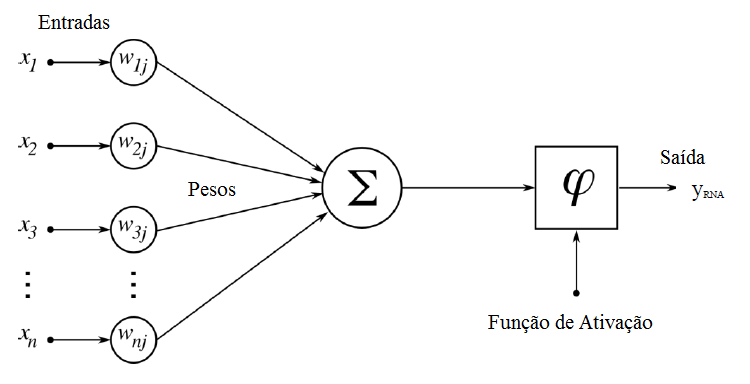
\includegraphics[scale=0.4]{images/Figura-1-neuronio-artificial.png}
\caption{Exemplo do modelo perceptron \cite{imagemperceptron}.}
\label{fig: perceptron}
\end{figure}

O modelo do perceptron, demonstrado na figura \ref{fig: perceptron}, é composto por algumas características principais: Um número $n$ de entradas, em que cada entrada será ponderada por seu respectivo peso $w$, e um termo de viés \(b\) (\textot{bias}). O funcionamento desse neurônio se inicia com uma combinação linear, que é a soma ponderada das entradas $x$ e dos pesos $w$, essa operação pode ser representada como: \(z = w_1  x_1 + ... + w_n  x_n\)  . O resultado dessa operação $(z)$ é passado então a uma função de ativação . Essa função de ativação tem a capacidade de amplificar o aprendizado desses sistemas, já que é essa função que determina se o neurônio será ativado ou não. Essa função de ativação é responsável por aplicar uma transformação não linear à saída da primeira operação, resultando na operação final representada por \(  \sigma  = f(z + b)\) , em que $b$ é termo de viés e $z$ o resultado do somatório \cite{haykin2009neural}. 


Considerando o entendimento do perceptron, a arquitetura baseada em redes neurais é dividida em basicamente três partes: A camada inicial, essa camada é responsável por receber os dados de entrada; as camadas ocultas, conhecidas também como \textit{hidden layers}, em que as informações são processadas, e a camada de saída, em que é gerado o valor de saída da rede. Além das redes neurais serem compostas por camadas de neurônios, cada neurônio em uma camada está conectado com todos os neurônios da camada seguinte, logo temos a formação de uma rede \gls{mlp}. Para análise de imagens, uma arquitetura que tem se mostrado muito eficiente é a rede neural convolucional (\gls{cnn}), essa arquitetura segue a mesma lógica dos modelos baseados em redes neurais, porém com um adicional, as convoluções. 

A convolução é um processo de filtragem espacial (plano que contém os pixels da imagem), que consiste em aplicar o somatório do produto entre duas matrizes, a imagem e uma máscara ao longo da região que estas se sobrepõem, sendo a imagem uma função bidimensional \( f(i,j)\), em que \(i\) e \(j\) são as coordenadas, e a amplitude de $f$ em qualquer par de coordenadas se refere a intensidade de cor naquele ponto, já a máscara uma matriz de tamanho variado \cite{gonzalez2008digital}. 

\begin{figure}[h]
    \centering
    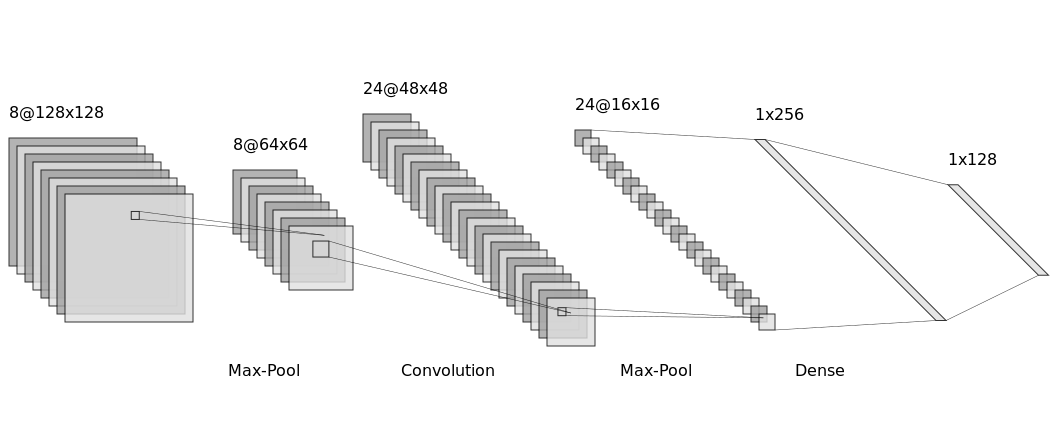
\includegraphics[scale=0.4]{images/redeconv.png}
    \caption{Exemplo rede neural convolucional.}
    \label{fig: cnn}
\end{figure}


As redes convolucionais, que seguem o modelo apresentado na figura \ref{fig: cnn}, geralmente recebem como entrada imagens e podem fazer extração de características e classificações a partir desses dados. Em casos de diagnóstico médico feito a partir da avaliação visual, como uma parte do diagnóstico da psoríase, por exemplo, o uso desses modelos seria adequado.

Uma alternativa à abordagem da \gls{cnn} é a arquitetura de \textit{Visual Transformers}. Essa arquitetura utiliza o algoritmo de \textit{Transformers} (figura \ref{fig:transformer-arch}) para análise de imagens, os \textit{transformers}, foram inicialmente propostos por \citeonline{Vaswani}. Diferente dos modelos recorrentes da época, que processavam informações de forma sequencial, o que impedia a paralelização eficiente dentro dos exemplos de treinamento em sequências longas e limitava o agrupamento de dados, o \textit{Transformer} abandona a recorrência. Em vez disso, ele se baseia inteiramente em um mecanismo de atenção para capturar dependências globais entre as entradas e saídas. 
Essa abordagem permitiu uma paralelização significativamente maior durante o treinamento e estabeleceu novos patamares de desempenho em tarefas como a tradução automática.

% Uma alternativa a abordagem da \gls{cnn} é a arquitetura de \textit{Visual Transformers}, essa arquitetura utiliza como base um algoritmo de atenção, a proposta inicial desse algoritmo tinha como objetivo propor uma solução aos modelos recorrentes da época para tarefas de tradução, esses outros modelos da época tinham uma natureza sequencial, o que impedia a paralelização dentro dos exemplos de treinamento \cite{Vaswani}. 

\begin{figure}
  \begin{minipage}[b]{0.6\textwidth}
    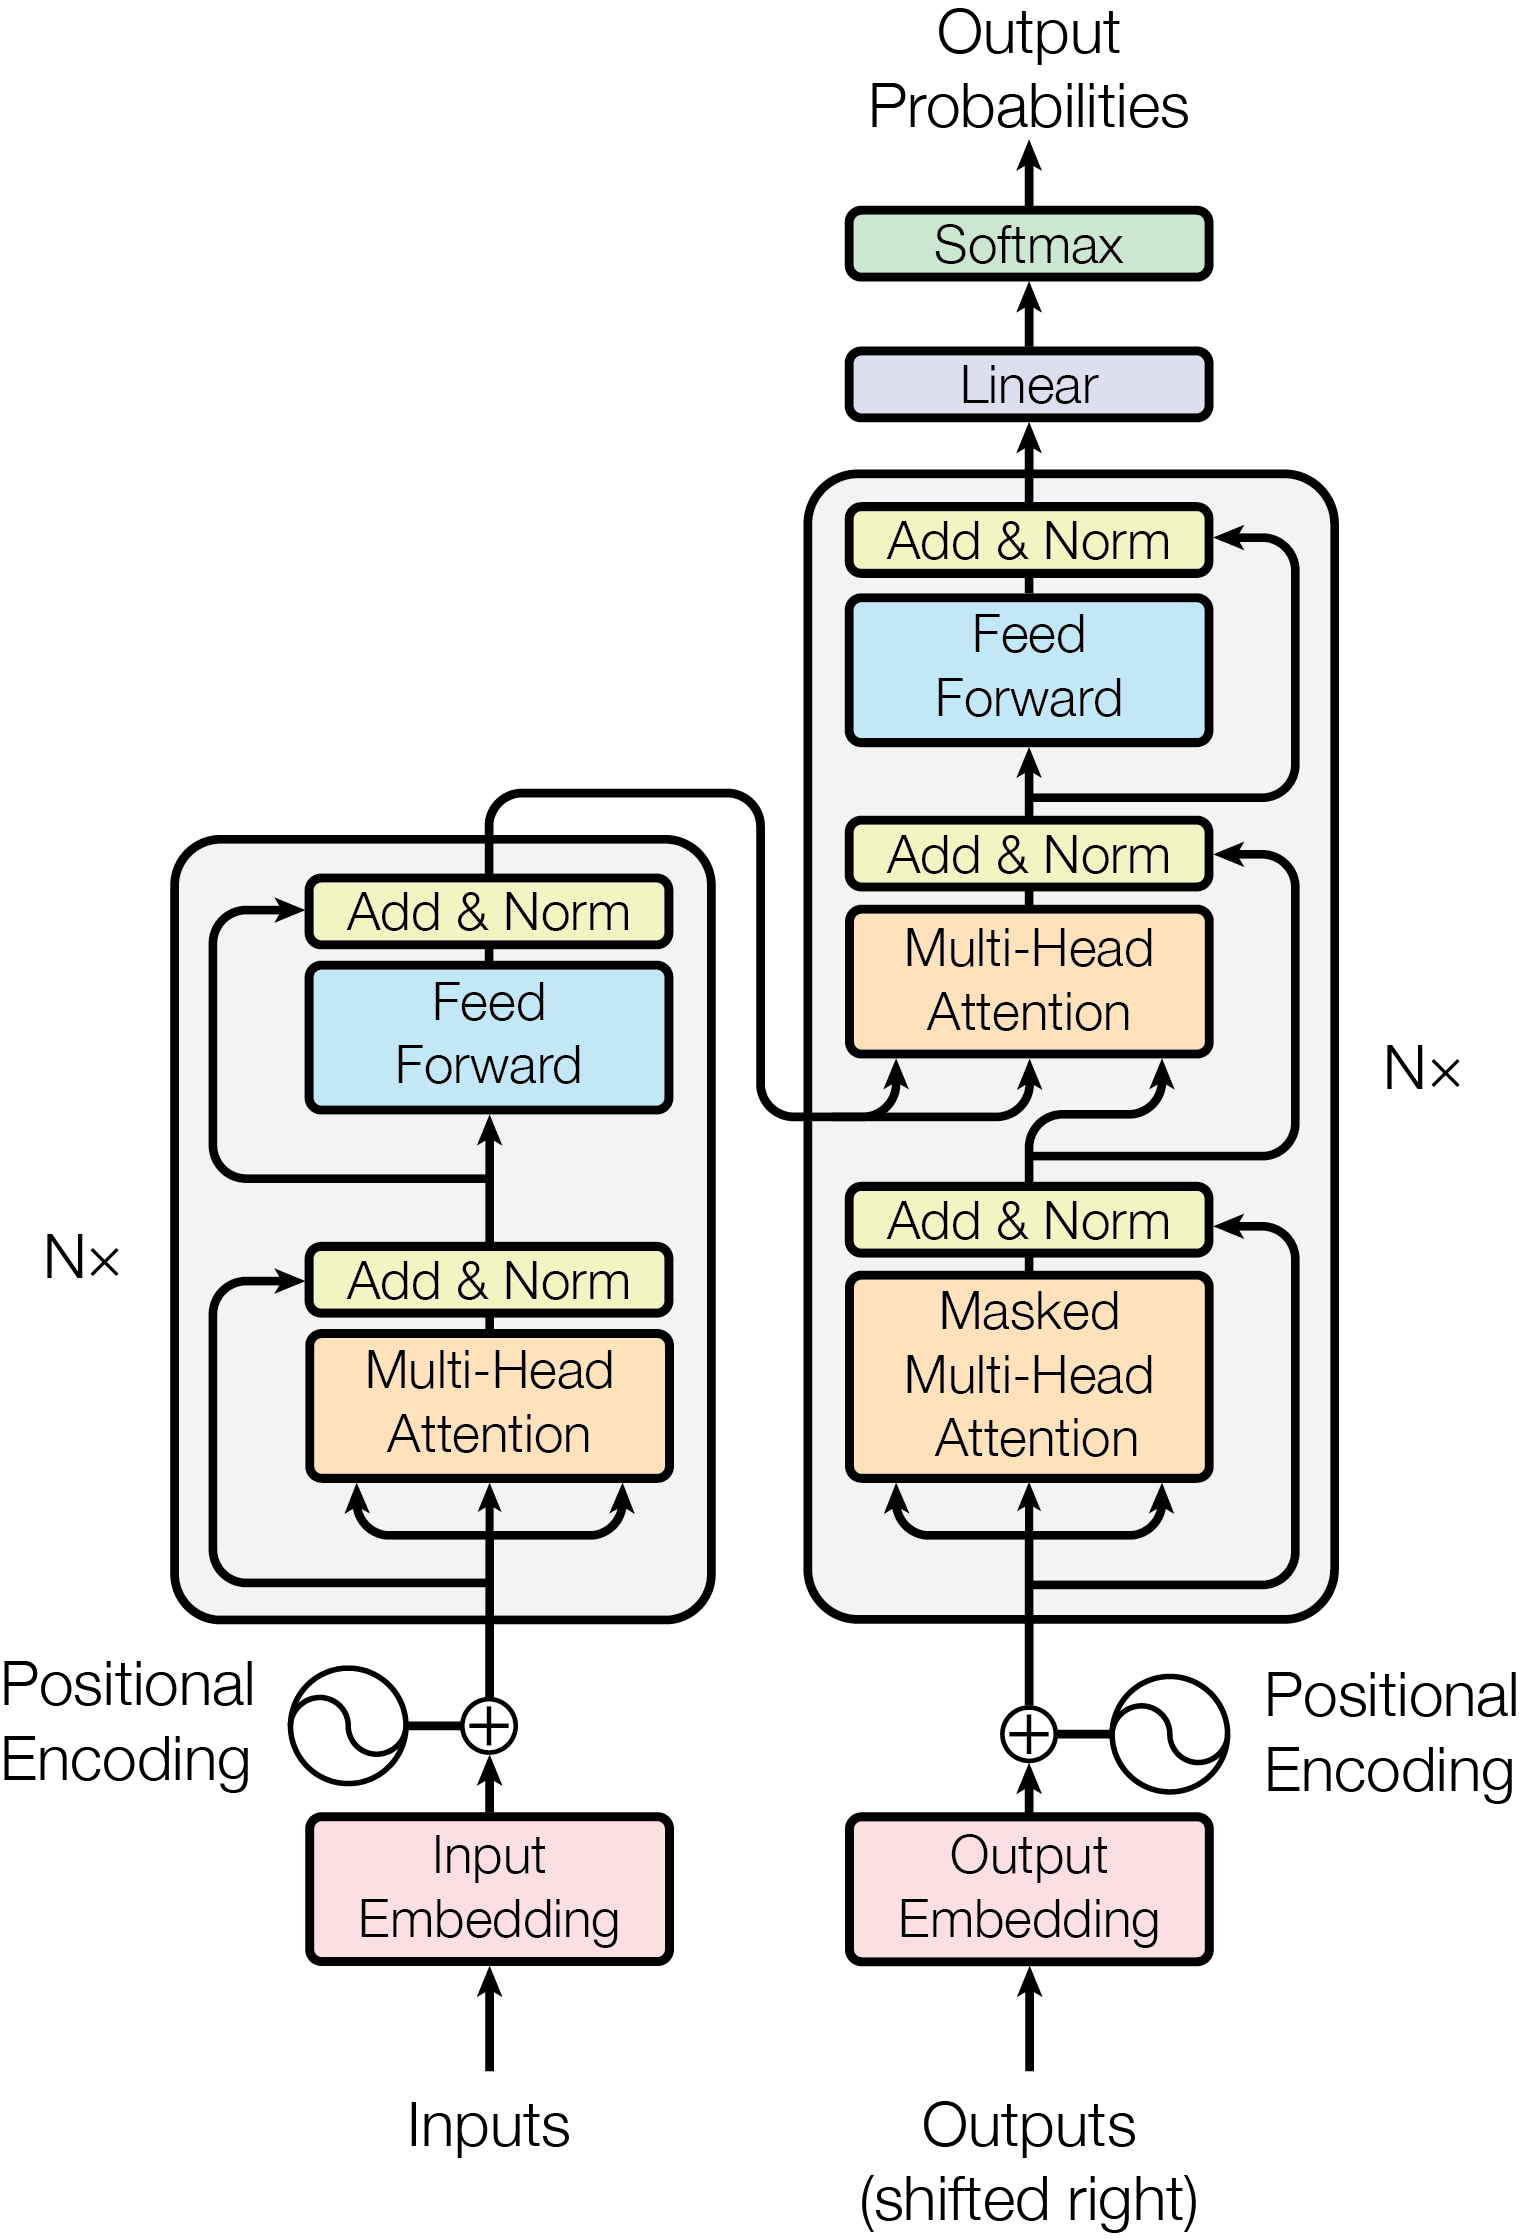
\includegraphics[scale=0.5]{images/ModalNet-21}
    \caption{Arquitetura do transformer. (\citeonline{Vaswani})}
    \label{fig:transformer-arch}
  \end{minipage}
  \begin{minipage}[b]{0.5\textwidth}
    \centering
    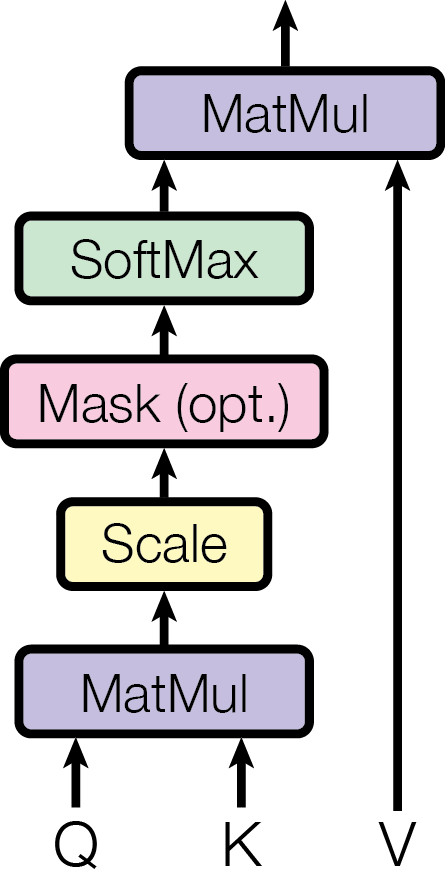
\includegraphics[scale=0.7]{images/ModalNet-19}
    \caption{Scaled Dot-Product Attention. (\citeonline{Vaswani})}
    \label{fig:dot-att}
  \end{minipage}
\end{figure}

\citeonline{Vaswani} define o mecanismo de autoatenção (\textit{self-attention}), demonstrado na figura \ref{fig:dot-att}, como um algoritmo que permite que o modelo pese a importância de diferentes partes da sequência de entrada ao gerar uma representação para cada elemento da sequência. As entradas são recebidas como vetores. Ao processar esse vetor, o modelo compara diretamente com todos os outros vetores na sequência de entrada simultaneamente em uma única camada, o que possibilita a paralelização, e determina quais são as mais relevantes para entender o contexto daquele elemento específico, diferentemente da \gls{cnn}, que consideram apenas as informações que se encontram no mesmo espaço do filtro definido, ou seja, contexto local. 
 Esse processo é realizado calculando scores de similaridade entre os elementos, permitindo que as dependências de longo alcance sejam capturadas de forma eficaz, sem as limitações sequenciais dos modelos recorrentes.

% \begin{figure}
%   \centering
%   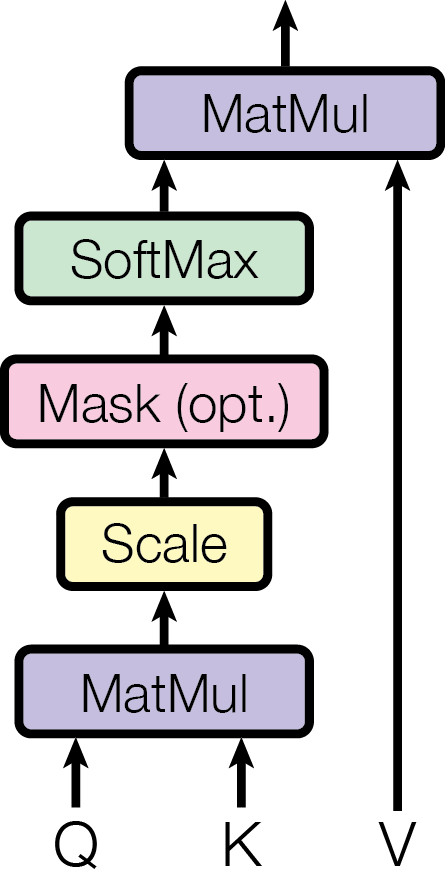
\includegraphics[scale=0.6]{images/ModalNet-19}
%   \caption{Scaled Dot-Product Attention.}
%   \label{fig:dot-att}
% \end{figure}
%
% Model overview. We split an image into fixed-size patches, linearly embed each of them, add position embeddings, and feed the resulting sequence of vectors to a standard Transformer encoder. In order to perform classification, we use the standard approach of adding an extra learnable classification token to the sequence. - peguei do artigo original
  
Os \textit{Visual Transformers} (figura \ref{fig:vit-arch}), por sua vez, dividem as imagens em patches de tamanhos fixos, diferentemente das \gls{cnn}s que processam pixels diretamente ou por meio de filtros convolucionais. Cada um desses patches é vetorizado e a esses vetores são adicionados embutimentos de posição (\textit{position embeddings}), para preservar a informação espacial original da imagem, após essa operação, essa sequencia passa por um \textit{encoder} padão que utiliza o algoritmo de atenção para aprender os padrões daquela sequência e as relações entre os diferentes patches da imagem. Para realizar tarefas de classificação, como a detecção de doenças de pele, um token de classificação extra, que é treinável, é adicionado à sequência, e sua saída final é usada para a previsão \cite{Dosovitskiy}.
\newline
\newline
\newline

% Imagem do artigo sobre visual transformers
\begin{figure}[h]
  \centering
    \begin{tabular}{c}
      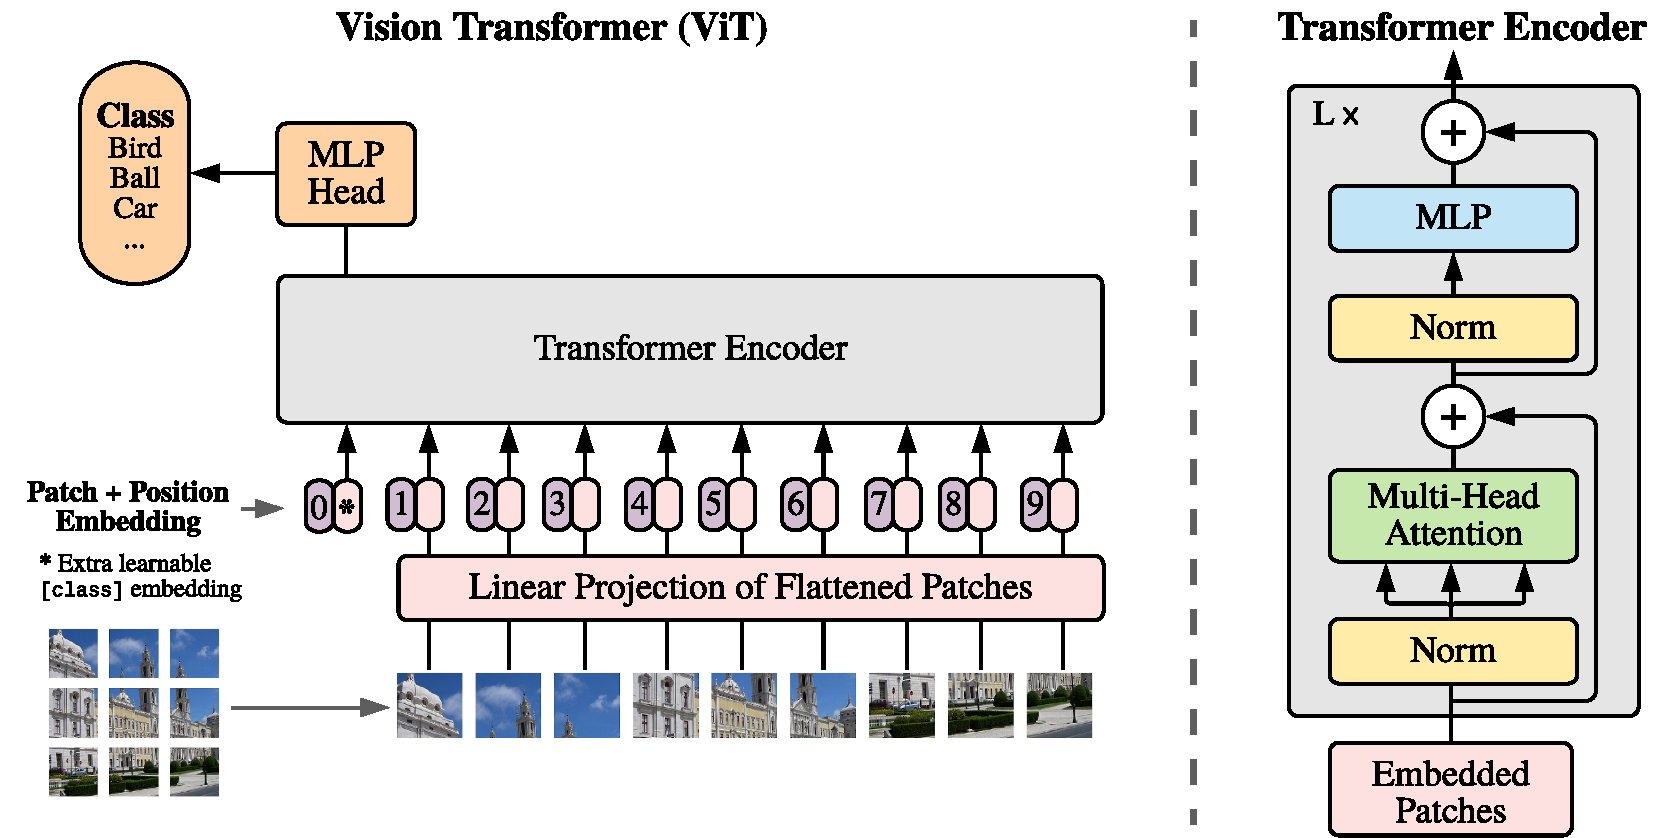
\includegraphics[scale=0.4]{images/model_scheme.pdf}
    \end{tabular}
    \caption{The Visual Transformer. (\citeonline{Dosovitskiy})}
    \label{fig:vit-arch}
\end{figure}

\subsection{Sobre Sistemas CAD}

Os primeiros estudos sobre análise quantitativa de imagens médicas por computador foram relatados na década de 1960. Porém, nos anos 80 surgiu uma nova abordagem, que assume que os sistemas CAD podem ser utilizados pelos profissionais da saúde como ferramenta e não para substituí-los. Assim, o objetivo principal desses sistemas é que a saída do CAD seja como uma “segunda opinião” para os médicos, para que estes façam a avaliação final. Nesse sentido, o uso dos sistemas CAD permite uma melhora na avaliação final em diferentes cenários, caso o médico esteja menos confiante sobre sua avaliação, a saída desse sistema tem a intenção de apoiar a avaliação final; e em uma situação onde o médico está mais confiante de sua avaliação, ele pode “descartar” a saída do computador. Alguns estudos afirmam que os sistemas CAD não precisam necessariamente se igualar ou superar a precisão na classificação em comparação aos profissionais na área da saúde, porém é importante ressaltar que quanto maior for o desempenho da máquina, melhor será o resultado final combinado \cite{DOI2007198}.

Para auxiliar na definição da metodologia do projeto de pesquisa, foi realizado um levantamento do estado da arte para as técnicas de classificação com imagens médicas. O processo de levantamento bibliográfico considerou o levantamento de artigos científicos nas bases científicas MDPI, IEEE, Elsevier e Scopus. Para realizar a busca dos artigos, foram utilizadas as palavras-chaves: “CAD”, “Computer Aided System”, “CAD convolution”, “psoriasis”, “CAD psoriasis”. Foram levantados 21 artigos considerando o filtro por título e resumo; dos quais, 13 foram detalhadamente analisados, com destaque para os trabalhos de Li (2020), Brinker (2019) e Doi (2007).

Li (2020), apresentou em sua pesquisa um sistema CAD para o diagnóstico de câncer de pâncreas. Nesse sistema, o autor utilizou um algoritmo baseado em support vector machine (SVM). Além desse algoritmo, o autor utilizou outras técnicas como o algoritmo LASSO, técnica de regularização usada principalmente para evitar o sobre ajuste do modelo e ajudar a selecionar as características importantes, e também propôs um modelo utilizando ensemble, que visa trazer mais robustez e melhorar a precisão do sistema através da construção e combinação de vários modelos. O algoritmo de ensemble usado para esse sistema foi o algoritmo bagging (bootstrap aggregating); nesse algoritmo várias subamostras são geradas aleatoriamente a partir do conjunto de dados original, com repetição e as previsões dos modelos individuais são combinadas para gerar uma previsão final. Esse sistema CAD atingiu uma precisão de 91.63\% para os dados na classe “Normal Stage - IV”, essa classe representa o estágio mais avançado da doença.

Já \citeonline{BRINKER201911}, apresentou em sua pesquisa um sistema CAD voltado para dermatologia, o modelo proposto superou dermatologistas na classificação de imagens de melanoma. Em seu trabalho, Brinker utilizou apenas imagens com uma qualidade avaliada como excelente, boa ou suficiente  pelos dermatologistas que participaram da pesquisa. O sistema CAD proposto foi desenvolvido usando uma arquitetura de redes neurais já conhecida, a ResNet50 e os dados vieram de fontes open-source (código aberto) e comprovados por biópsia. Considerando um intervalo de confiança (CI) de 95\%, após o treinamento do modelo, este atingiu uma sensibilidade de 82.3\% (95\% CI: 78.3–85.7\%) e especificidade de 77.9\% (95\% CI: 73.8–81.8\%), já os dermatologistas atingiram uma sensibilidade de 67.2\% (95\% CI: 62.6–71.1\%) e especificidade de 62.2\% (95\% CI: 57.6–66.9\%).


Ainda no contexto dermatológico, \citeauthor{DASH2020106240} apresenta um sistema CAD totalmente integrado, que é composto por três estágios: classificação, segmentação e avaliação da severidade da lesão. No primeiro estágio, o sistema é baseado numa arquitetura de redes convolucionais chamada de VGG-16, composta de 13 camadas convolucionais e 3 camadas totalmente conectadas. Neste trabalho, algumas alterações foram feitas nesse modelo, como a remoção de camadas “redundantes”, com o objetivo de reduzir a quantidade de parâmetros, tornando assim essa rede mais eficiente computacionalmente. A primeira parte do trabalho, que compõe a rede convolucional para classificação da doença, atingiu uma acurácia de 93.76\%.


Como já visto anteriormente, em sua grande maioria, esses sistemas são construídos para lidar com dados não estruturados, que é o caso de imagens. A visão humana, diferente dos computadores, é limitada à banda visual do \ac{EM}, já os aparelhos de processamento de imagens cobrem quase todo o espectro eletromagnético (EM), variando de ondas gama a ondas de rádio; basicamente esses dispositivos são capazes de trabalhar com imagens geradas por fontes que os seres humanos não estão acostumados a associar, entre esses tipos de fonte, estão: imagens geradas por ultrassons, microscopia eletrônica e imagens gerada por computador \cite{gonzalez2008digital}. 


Há uma grande vantagem na aplicação da visão computacional nesse setor, que por sua vez, estuda diferentes técnicas para trabalhar com imagens, como por exemplo, os já citados modelos de classificação, além de técnicas de extração de características, detecção de bordas, entre outras. Entre essas diversas técnicas, destacam-se os modelos baseados na arquitetura de redes neurais \cite{DOI2007198}.


Do mesmo modo que a visão computacional avança com suas técnicas na área da saúde, outra área que também se beneficia é o processamento digital de imagens, que possui uma relação muito forte com a visão computacional. Essa área de estudo está ligada principalmente com os conceitos de filtragem, transformações geométricas e restauração de imagens. O objetivo desses tratamentos nas imagens é prepará-las para análises posteriores, de modo a oferecer as técnicas necessárias para pré-processar e manipular imagens, antes de “alimentar” esses dados nas redes convolucionais \cite{gonzalez2008digital}.



  \section{Metodologia}

O presente projeto tem a intenção de desenvolver um sistema \acs{\acs{CNN}}, que será formado a partir de uma arquitetura de \acs{IA} híbrida, em que uma parte desse modelo terá a tarefa de lidar com a base de dados de imagens que será fornecida pela \ac{FMABC}, sendo essa base composta de imagens de pacientes brasileiros afetados pela psoríase, e a outra parte lidar com os dados clínicos, como por exemplo exames de sangue PCR e velocidade de hemossedimentação, ambos os exames podem sofrer alteração em casos inflamatórios, que também será fornecido pela \acs{FMABC} em anuência do comitê de ética em pesquisa da \acs{FMABC}. A intenção dessa proposta é que a combinação de diferentes análises e informações traga um aumento na precisão desse tipo de sistema, fornecendo um suporte à tomada de decisão. Efetivamente, será implementada uma solução de ponta a ponta, que exigirá desde técnicas para o tratamento e preparo dos dados, até soluções para o refinamento do modelo de \acs{IA}.


A partir dos conceitos de redes neurais artificiais e \textit{transformers}, fica mais claro entender a construção dos modelos de \acs{IA}, que seguem um certo padrão, esse padrão é conhecido como \textit{pipeline}. Os \textit{pipelines} de \acs{IA} envolvem todo o fluxo de atividades necessárias para o funcionamento apropriado do modelo. De modo genérico, este fluxo geralmente começa com atividades relacionadas à extração, transformação e carregamento dos dados, processo conhecido como \ac{ETL}; no caso de modelos de \acs{IA} voltados a visão computacional, essa fase utiliza técnicas para preparar essas imagens a um modelo de \acs{IA}, geralmente envolvendo atividades relacionadas ao processamento digital de imagens. Além das transformações nas imagens é necessário realizar uma estratificação dos dados, uma parte deve ser separada para o treinamento da rede, enquanto a outra deve ser exclusivamente voltada para a validação da rede. A etapa seguinte envolve o treinamento da rede, essa etapa exige diferentes técnicas para o sucesso do modelo, entre essas técnicas estão a escolha de um algoritmo de otimização adequado ao problema, o uso de uma função de perda apropriada, ajuste correto dos hiperparâmetros da rede e número de épocas no treinamento.

Foram estudadas diversas alternativas de parametrização da rede proposta com o objetivo de aumentar a precisão dos diagnósticos, dentre as técnicas aplicadas, se destaca o \textit{GridSearch} . O pipeline desse projeto pode ser dividido inicialmente em algumas etapas, começando com a construção de uma aplicação para a extração, transformação e carregamento (\acs{ETL}) dos dados, em que, serão realizadas todas as atividades necessárias para garantir que esses dados estejam seguros e disponíveis, seguindo com técnicas de aumento da base de dados de imagens para o treinamento do modelo de \acs{CNN}, esta fase irá exigir um estudo profundo do conjunto de dados de imagens, pois as transformações aplicadas nas imagens terão impacto direto em como a \acs{CNN} irá desempenhar futuramente. Transformações como o tamanho da imagem, conversão de domínio de cores, rotação das imagens, entre outras diversas transformações serão avaliadas neste momento. Essas técnicas também possibilitam que o modelo seja treinado com uma base de dados maior e mais diversificada, aumentando sua generalização. Além da aplicação de técnicas de aumento da base será necessário utilizar metodologias para a estratificação dos dados, o método utilizado será de validação cruzada k-pastas estratificado para avaliar o desempenho do modelo. Em seguida, será realizado o desenvolvimento e treinamento de um modelo de \acs{CNN}, nesta fase serão estudadas diversas arquiteturas de redes convolucionais e aplicações dessas arquiteturas na área da saúde, além de alternativas para equilibrar a precisão do modelo e sua quantidade de parâmetros, um dos fatores que determina o impacto computacional da rede neural. Por fim, o modelo será avaliado utilizando diferentes métodos estatísticos, como z-score, acurácia, precisão, sensibilidade, especificidade e perda.

Já a segunda parte compõe a construção e treinamento de um modelo de \acs{MLP}, que trabalhará em conjunto com a \acs{CNN}, portanto, a saída da \acs{CNN} irá compor um dos parâmetros de entrada no \acs{MLP}. Será necessário integrar uma rede \acs{MLP} ao modelo de classificação de imagens. Além das técnicas já previstas como validação cruzada e avaliação do modelo, também será necessário analisar e tratar os dados clínicos e construir a integração dos dois modelos. Será realizado um estudo com os resultados de desempenho desses modelos de forma individual e dos modelos em conjunto, além de uma avaliação da viabilidade para a preparação de tal sistema em um produto.
%
% %\begin{table}[h!]
\centering
\setlength{\arrayrulewidth}{0.8pt}
\setlength{\tabcolsep}{5pt}
\renewcommand{\arraystretch}{1.2}


\small
\centering\begin{tabular}{|p{9cm}|*{11}{c|}}
\hline
\textbf{Atividades} & \multicolumn{11}{c|}{\textbf{Meses}} \\
\hline
  &
\textbf{1} & \textbf{2} & \textbf{3} & \textbf{4} & \textbf{5} & \textbf{6} & \textbf{7} & \textbf{8} & \textbf{9} & \textbf{10} & \textbf{11} \\ 
\hline
Criação de uma pipeline de dados para o armazenamento e tratamento dos dados & x & x &   &   &   &   &   &   &   &   &   \\ \hline
Análise detalhada das técnicas em sistemas CAD                              &   & x &   &   &   &   &   &   &   &   &   \\ \hline
Construção de uma prova de conceito do modelo de CNN para avaliar a viabilidade das técnicas escolhidas &   & x &   &   &   &   &   &   &   &   &   \\ \hline
Análise dos resultados da prova de conceito do modelo e definição das técnicas para a construção do modelo &   &   & x &   &   &   &   &   &   &   &   \\ \hline
Construção do modelo de CNN                                                &   &   &   & x & x &   &   &   &   &   &   \\ \hline
Avaliação do modelo de CNN e ajuste de hiperparâmetros                     &   &   &   &   & x & x &   &   &   &   &   \\ \hline
Construção da prova de conceito de um modelo de MLP                        &   &   &   &   &   & x &   &   &   &   &   \\ \hline
Análise de resultados da prova de conceito do modelo de MLP e definição das técnicas para o desenvolvimento do modelo de MLP &   &   &   &   &   &   & x &   &   &   &   \\ \hline
Construção do modelo MLP                                                   &   &   &   &   &   &   & x & x &   &   &   \\ \hline
Testes com o modelo e ajustes de hiperparâmetros                           &   &   &   &   &   &   &   & x & x &   &   \\ \hline
Análise de precisão do modelo em relação ao modelo de CNN                  &   &   &   &   &   &   &   &   & x & x &   \\ \hline
Análise de viabilidade do sistema                                          &   &   &   &   &   &   &   &   &   & x &   \\ \hline
Elaboração de artigo científico com apresentação dos resultados            &   &   &   &   &   &   &   &   &   & x & x \\ \hline
Processo de submissão do artigo científico para periódico                  &   &   &   &   &   &   &   &   &   &   & x \\ \hline
\end{tabular}
\caption{Cronograma de atividades do desenvolvimento do projeto.}
\label{cronograma}
\end{table}




%
% Presente projeto tem característica quantitativa, visto que se enquadra nas definições de ser conseguido na busca de resultados exatos evidenciados por meio de variáveis preestabelecidas, em que se verifica e explica a influência sobre as variáveis, mediante análise da frequência de incidências e correlações estatísticas \cite{michelmetodologia}.
%
% O desenvolvimento do trabalho se divide em duas grandes áreas de atuação, Inteligência artificial, que atende todo o escopo do desenvolvimento do modelo de segmentação. E engenharia de software, que engloba os conteúdos necessários para o desenvolvimento do protótipo de software.
%
% \subsection{Do desenvolvimento do modelo}
%
% Conforme apresentado na seção anterior, a aplicação das técnicas de visão computacional na medicina tem se mostrado muito promisoras para o diagnóstico de doenças complexas e melhora na eficiência do diagnóstico clínico. A integração de diferentes dados, como exames laboratoriais e imagens médicas, possibilitará a construção de um sistema robusto, capaz de analisar diferentes tipos e grandes volumes de dados. A Figura \ref{fig:pipeline} ilustra, de forma abstrata, como será o funcionamento do sistema proposto.
%
% \begin{figure}[h]
%     \centering
%     
\includegraphics[scale=0.15]{images/pipeline2.png}
%     \caption{Pipeline do projeto}
%     \label{fig:pipeline}
% \end{figure}
%
% Cada fase do pipeline será projetada para realizar operações críticas para o resultado do modelo, buscando também maior desempenho e resiliência para esse sistema. Serão detalhadas cada uma das etapas.
%
% \subsubsection{Coleta dos dados}
%
% Essa etapa é responsável pela extração e organização dos dados, serão utilizadas técnicas de engenharia de dados para garantir que todo o processo de coleta dos dados seja seguro e consistente. Desta maneira, para assegurar esses objetivos, o sistema terá integração com dados de diversas fontes diferentes, essa integração para a coleta das informações será feita através de interfaces de programação de aplicação (\textit{API}), que possibilitará a automatização dessa fase. Para o desenvolvimento dessa etapa, serão empregadas a linguagem de programação python e a ferramenta \textit{spark} como recursos principais. No contexto deste estudo, a coleta foi realizada a partir de bancos de dados públicos médicos, o portal escolhido responsável pelas informações é o The Cancer Imaging Archive \cite{cancerimaging}, foram extraídos diferentes conjuntos de dados. 
%
% A figura \ref{fig:ex-dataset}, apresenta uma imagem retirada do conjunto fornecido pelo the Cancer Imaging Archive. Esse conjunto é composto por 610 imagens microscópicas de melioma múltiplo. A localização do câncer é nos ossos, as imagens possuem ampliação de 1000x, tendo as dimensões de 1126x874 pixels.
%
%
% \begin{figure}[h] % Ajuste largura
%     \centering
%     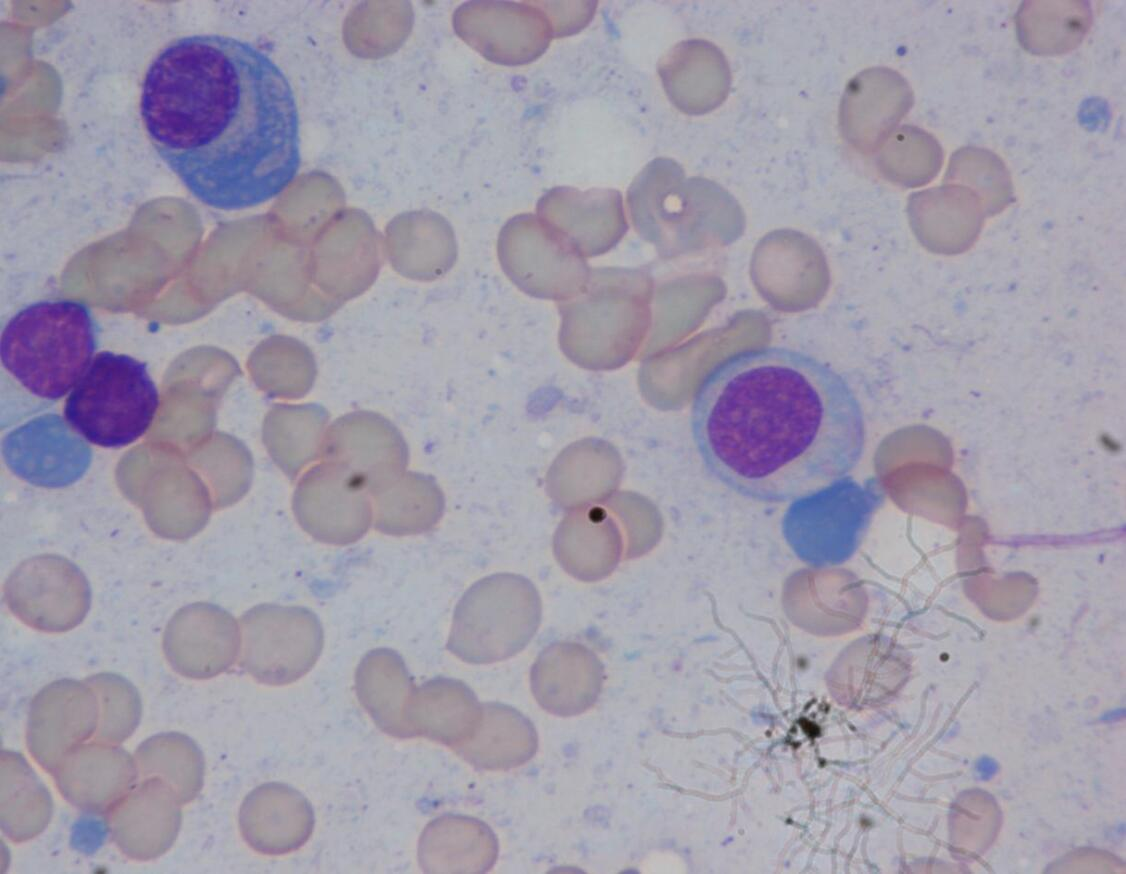
\includegraphics[width=0.3\textwidth]{images/datasetexample.jpg}
%     \caption{Imagem microscópica de câncer nos ossos}
%     \label{fig:ex-dataset}
% \end{figure}
%
% \subsubsection{Pré processamento}
%
% Após a etapa anterior, será necessário tratar as informações coletadas. Com isso, será aplicado operações como a limpeza de dados, que envolve a remoção de valores inconsistentes, ajuste de escalas de valores e codificação de variáveis categóricas, por exemplo. Além disso, para os dados de imagens, serão utilizadas técnicas de aumento de dados, para maior generalização do modelo. Também serão explorados técnicas de processamento digital de imagens, como regulagem de luminosidade e transformação para diferentes domínios de cor como YCbCr.
%
% \subsubsection{Extração de características}
%
% Antes de realizar o treinamento efetivo do modelo, será necessário extrair características a partir das imagens médicas, como textura, bordas e padrões. Durante a fase de extração de características, o principal objetivo é transformar os dados recebidos em representações que melhor capturam os padrões subjacentes e são mais informativas para o algoritmo de aprendizado. Para a seleção de características relevantes, técnicas como análise de correlação e análise de variância serão utilizados para apoio à seleção. Para os dados de imagens, a extração de características estará incorporada ao treinamento, visto que as camadas convolucionais têm a responsabilidade de aprender os padrões hierárquicos e abstratos.
%
% \subsubsection{Treinamento do modelo}
%
% Com todas as informações já preparadas, serão exploradas diferentes técnicas de convoluções para a segmentação das imagens microscópicas, como por exemplo a \textit{pixel-wise convolution}, uma técnica que possibilita a combinação de informações entre os canais de uma imagem. Será avaliado a possibilidade de utilizar técnicas de \textit{ensemble} nessa fase, de modo a combinar da melhor maneira os dados clínicos com as imagens microscópicas. Também será explorado técnicas para otimizar o treinamento, como ajuste da taxa de aprendizado de forma dinâmica entre as diferentes camadas de acordo com algumas métricas, como o erro das previsões. Para fins de melhora no desempenho, o treinamento do modelo também envolverá técnicas de computação paralela, com isso será possível um treinamento mais otimizado do sistema.
%
% \subsubsection{Avaliação do modelo}
%
% Como etapa final, a avaliação do modelo é responsável por aplicar métodos estatísticos para consolidar os resultados das etapas previstas. Conforme os resultados desses métodos, será possível analisar se o desempenho do modelo está de acordo com o esperado. Dentre as técnicas mais comuns, serão utilizadas métricas como acurácia, definida pela fórmula 
% \begin{equation}
%   acurácia = \frac{VP +VN}{VP + FN + VN + FP} \; ,
%     \label{eq: acuracia}
% \end{equation}
% \\
% em que \(VP\) é a quantidade de verdadeiros positivos; \(VN\) é a quantidade de verdadeiros negativos; \(FN\) é a quantidade de falsos negativos e \(FP\) é a quantidade de falsos positivos. Também será utilizado a métrica de avaliação precisão, determinada pela fórmula:
%
% \begin{equation} 
%   precisão = \frac{VP}{VP + VF} \; ,
%   \label{eq: precisao}
% \end{equation}
%  \\
% E por último, uma métrica de avaliação chamada sensibilidade, estabelecida pela fórmula:
%
% \begin{equation}
% sensibilidade = \frac{VP}{VP + FN} \; ,
%   \label{eq: sensibilidade}
% \end{equation}
% \\
% Paralelamente, todas as fases irão contar com um minucioso registro de todas as ações para monitoramento do sistema. Além disso, serão implementados mecanismos de auditoria para garantir a rastreabilidade das operações realizadas, promovendo maior transparência e confiabilidade. Esse registro incluirá não apenas informações sobre as decisões tomadas pelo sistema, mas também os dados utilizados em cada etapa, possibilitando a análise detalhada de possíveis erros ou inconsistências e facilitando ajustes futuros para otimização do desempenho.
%
% \subsection{Do protótipo da aplicação web}
%
% Para o uso desse modelo em um potencial sistema, serão utilizados diferentes componentes de tecnologia, envolvendo áreas como arquitetura de software, desenvolvimento backend, computação em nuvem, e conceitos de computação distribuída, a fim de projetar um sistema que seja resiliente, distribuído e escalável.
%
% \subsubsection{Da arquitetura do protótipo}
% O sistema proposto adota uma arquitetura baseada em microsserviços, modelo arquitetural que promove o desacoplamento dos componentes, permitindo evolução independente de cada serviço. Essa abordagem facilita a escalabilidade horizontal, melhora a manutenção e possibilita a implementação de diferentes tecnologias conforme as necessidades específicas de cada módulo. Além disso, a divisão funcional dos serviços contribui para um gerenciamento mais eficiente da infraestrutura e do processamento de dados, garantindo maior flexibilidade e modularidade no desenvolvimento e na implantação.
%
% \subsubsection{Da definição dos protocolos de comunicação}
% Além da definição da arquitetura desse protótipo, também serão explorados protocolos de comunicação de alta desempenho para garantir maior confiabilidade e reduzir latência entre os serviços. Protocolos como o \textit{Remote Procedure Call} (RPC) serão utilizados para garantir essa comunicação eficiente entre serviços. O RPC possui algumas vantagens em relação a outros protocolos, dentre elas estão a serialização binária e suporte a conexões persistentes, características que garantem um \textit{payload} menor sendo trafegado, reduzindo a latência e otimizando o desempenho \cite{Niswar2024}. 
%
% \subsubsection{Do monitoramento do protótipo}
% A fim de avaliar o desempenho do sistema proposto, serão implementadas estratégias de monitoramento para análise detalhada do comportamento da aplicação em diferentes cenários de carga e uso. Ferramentas como Prometheus e Grafana serão empregadas para coleta de métricas e visualização do desempenho dos microsserviços em tempo real, permitindo identificação de potenciais gargalos e otimizações. Além disso, serão adotadas técnicas de observabilidade avançadas, como logs estruturados e rastreamento distribuído com OpenTelemetry, possibilitando uma análise aprofundada das interações entre os serviços e assegurando uma resposta eficiente a eventuais falhas.
%
% % --- Poderia ficar nos objetivos? ---
% % Além do desenvolvimento de um modelo que seja capaz de segmentar imagens microscópicas de células com alta precisão, esse trabalho também propõe a aplicação desse modelo num sistema destinado a uso médico. 


  % \section{Cronograma}

Para alcançar o objetivo proposto neste projeto de pesquisa, os objetivos específicos traduzidos em tarefas de desenvolvimento serão desenvolvidos. O cronograma descrito na tabela \ref{cronograma} apresenta a distribuição dessas atividades no tempo.

\begin{table}[h!]
\centering
\setlength{\arrayrulewidth}{0.8pt}
\setlength{\tabcolsep}{5pt}
\renewcommand{\arraystretch}{1.2}


\small
\centering\begin{tabular}{|p{9cm}|*{11}{c|}}
\hline
\textbf{Atividades} & \multicolumn{11}{c|}{\textbf{Meses}} \\
\hline
  &
\textbf{1} & \textbf{2} & \textbf{3} & \textbf{4} & \textbf{5} & \textbf{6} & \textbf{7} & \textbf{8} & \textbf{9} & \textbf{10} & \textbf{11} \\ 
\hline
Criação de uma pipeline de dados para o armazenamento e tratamento dos dados & x & x &   &   &   &   &   &   &   &   &   \\ \hline
Análise detalhada das técnicas em sistemas CAD                              &   & x &   &   &   &   &   &   &   &   &   \\ \hline
Construção de uma prova de conceito do modelo de CNN para avaliar a viabilidade das técnicas escolhidas &   & x &   &   &   &   &   &   &   &   &   \\ \hline
Análise dos resultados da prova de conceito do modelo e definição das técnicas para a construção do modelo &   &   & x &   &   &   &   &   &   &   &   \\ \hline
Construção do modelo de CNN                                                &   &   &   & x & x &   &   &   &   &   &   \\ \hline
Avaliação do modelo de CNN e ajuste de hiperparâmetros                     &   &   &   &   & x & x &   &   &   &   &   \\ \hline
Construção da prova de conceito de um modelo de MLP                        &   &   &   &   &   & x &   &   &   &   &   \\ \hline
Análise de resultados da prova de conceito do modelo de MLP e definição das técnicas para o desenvolvimento do modelo de MLP &   &   &   &   &   &   & x &   &   &   &   \\ \hline
Construção do modelo MLP                                                   &   &   &   &   &   &   & x & x &   &   &   \\ \hline
Testes com o modelo e ajustes de hiperparâmetros                           &   &   &   &   &   &   &   & x & x &   &   \\ \hline
Análise de precisão do modelo em relação ao modelo de CNN                  &   &   &   &   &   &   &   &   & x & x &   \\ \hline
Análise de viabilidade do sistema                                          &   &   &   &   &   &   &   &   &   & x &   \\ \hline
Elaboração de artigo científico com apresentação dos resultados            &   &   &   &   &   &   &   &   &   & x & x \\ \hline
Processo de submissão do artigo científico para periódico                  &   &   &   &   &   &   &   &   &   &   & x \\ \hline
\end{tabular}
\caption{Cronograma de atividades do desenvolvimento do projeto.}
\label{cronograma}
\end{table}






% --- Imagem do cronograma

%\begin{figure}[h]
%    \centering
%    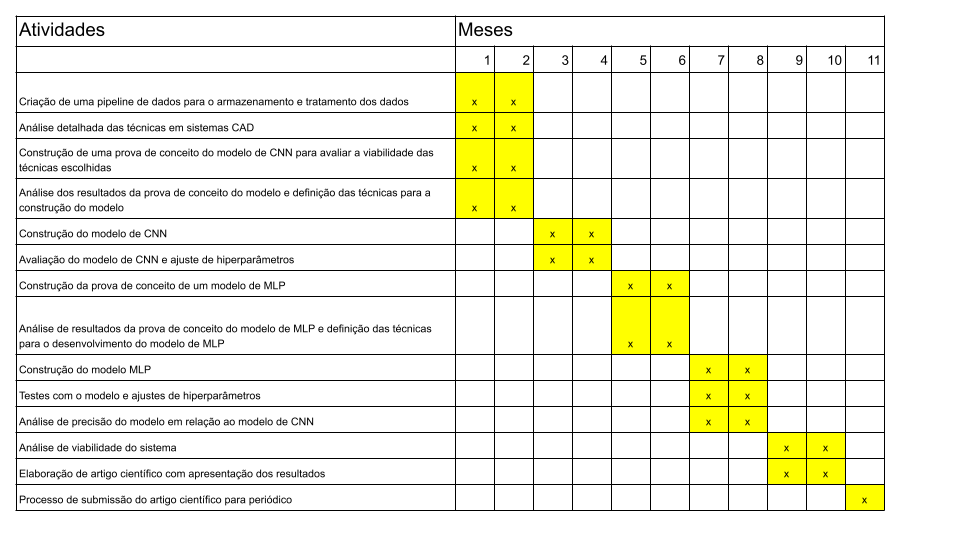
\includegraphics[scale=0.5]{images/Cronograma.png}
%    \caption{Tabela 1: Cronograma de atividades do desenvolvimento do projeto}
%    \label{fig:enter-label}
%\end{figure}



  \section{Resultados e Discussão}

A rede treinada apresentou resultados relevantes e muito promissores. Um dos principais desafios encontrado durante o processo de desenvolvimento foi a complexidade de trabalhar com o dataset, além do pré-processamento, també foi necessário a remoção de certas imagens que não estavam adequadas para o treinamento da rede, devido a diversos fatores externos, como por exemplo qualidade da foto. Mesmo em um ambiente controlado não havia um padrão da maneira como os dados eram gerados, portanto diversas imagens necessitavam de análise individual. A tabela \ref{tab:db-table} indica algumas informações sobre o dataset utilizado para o treinamento do modelo após o pré-processamento. 

Após todo o tratamento do dataset houve uma diminuição expressiva do volume da base de dados, um pouco mais de 50\% de redução, esse fator também gerou outros desafios durante a fase de treinamento, como a falta de elementos representativos. A imagem abaixo é um exemplo do resultado final sendo alimentado na rede.

\newline
\begin{table}[h]
  \centering
  \label{tab:db-table}
  \begin{tabular}{|l|l|l|}
  \hline
  \multicolumn{1}{|c|}{\textbf{Label}} & \multicolumn{1}{c|}{\textbf{Amostras}} & \multicolumn{1}{c|}{\textbf{Porcentagem}} \\ \hline
  Psoríase                             & 1019                                   & 45.1\%                                  \\ \hline
  Dermatite                            & 1239                                   & 54.9\%                                  \\ \hline
  \multicolumn{1}{|c|}{\textbf{Total}} & \multicolumn{1}{c|}{\textbf{2258}}     & \multicolumn{1}{c|}{\textbf{100\%}}     \\ \hline
  \end{tabular}
  \caption{Distribuição do dataset após o processo de curadoria.}
\end{table}

Apesar da redução do volume de dados, o modelo alcançou um desempenho satisfatório. A Tabela \ref{tab:resultados_metricas} resume as métricas de avaliação obtidas no conjunto de teste. Observa-se que a acurácia de XX\% e o F1-Score de YY\% indicam uma performance equilibrada, com a rede demonstrando robustez na distinção entre as classes.

\begin{table}[h]
  \centering
  \label{tab:resultados_metricas}
  \begin{tabular}{|l|c|}
  \hline
  \multicolumn{1}{|c|}{\textbf{Métrica}} & \textbf{Valor} \\ \hline
  Acurácia                               & XX\%           \\ \hline
  Precisão                               & YY\%           \\ \hline
  Revocação                              & ZZ\%           \\ \hline
  F1-Score                               & AA\%           \\ \hline
  \end{tabular}
  \caption{Resultados das métricas de avaliação do modelo no conjunto de teste.}
\end{table}

Além da avaliação quantitativa, a interpretabilidade do modelo foi investigada por meio da técnica de Grad-CAM. A Figura \ref{fig:gradcam} apresenta um mapa de calor que ilustra as regiões de uma imagem de psoríase nas quais o modelo concentrou sua atenção para realizar a classificação. A análise visual desta figura confirma que a rede não se baseia em ruídos ou artefatos da imagem, mas sim nas características morfológicas da área lesionada (destacada em vermelho), o que fortalece a confiança em seus resultados e valida sua aplicabilidade clínica como ferramenta de apoio ao diagnóstico.


Durante o treinamento e a avaliação foram utilizadas diferentes técnicas que possibilitassem a análise do desempenho do modelo, a figura demostra as áreas de interesse que o modelo analisou para a classificação da doença. A partir dessa figura, é possível compreender como o modelo foi capaz de relacionar o contexto da região vermelha (área lesionada) com a classificação da doença psoriase


\newpage



  \section{Conclusão}

Este trabalho apresentou o desenvolvimento de um sistema \gls{cad} para diagnóstico de psoríase vulgar baseado em \textit{Visual Transformers}, utilizando dados de pacientes brasileiros fornecidos pela \gls{fmabc}. O objetivo principal foi criar uma ferramenta de apoio ao diagnóstico capaz de distinguir entre psoríase vulgar e dermatite por meio de técnicas de visão computacional e processamento digital de imagens. Para atingir essa meta, foi implementado um \textit{pipeline} completo que envolveu desde a coleta e curadoria dos dados até o treinamento e avaliação de um modelo baseado na arquitetura \textit{Swin Transformers}. O modelo desenvolvido alcançou resultados promissores, com acurácia de 93,78\%, precisão de 92,11\%, revocação de 91,42\% e F1-Score de 91,76\%, demonstrando sua capacidade de classificação binária entre as duas condições dermatológicas estudadas.

Apesar dos resultados quantitativos satisfatórios, é fundamental destacar as limitações inerentes ao modelo, em grande parte, devido às características do dataset utilizado. A redução de mais de 50\% da base de dados original, embora necessária para garantir a qualidade das amostras, resultou em um volume limitado de imagens para o treinamento. 

Adicionalmente, as imagens foram capturadas em um ambiente controlado de laboratório universitário, o que as torna menos representativas de cenários clínicos reais, onde a variação de iluminação, qualidade da câmera e angulação é muito maior. Consequentemente, o modelo pode ter sua capacidade de generalização comprometida ao ser aplicado a imagens com características diferentes daquelas do conjunto de dados curado, como em um cenário de triagem em consultórios médicos. Tais limitações reforçam a necessidade de futuras pesquisas que utilizem um conjunto de dados mais diversificado, de maior volume e que simulem as condições do mundo real, a fim de aprimorar a robustez e a aplicabilidade clínica do modelo.

Apesar das limitações inerentes ao conjunto de dados, os resultados obtidos nesta pesquisa demonstram o potencial significativo do desenvolvimento de um sistema \gls{cad}.
A utilização de dados de pacientes brasileiros confere um valor estratégico ao modelo para a aplicabilidade em cenários clínicos nacionais. Além disso, este estudo serve como um ponto de partida para trabalhos futuros promissores. A evolução para um sistema capaz de realizar a segmentação automática da lesão ou a classificação da severidade da doença são direções de pesquisa que poderiam ampliar a funcionalidade e o impacto clínico da ferramenta.


  \renewcommand{\refname}{5 Referências}
\bibliographystyle{abntex2-alf}
\bibliography{Library}

\end{document}
